\begin{figure}[t!]
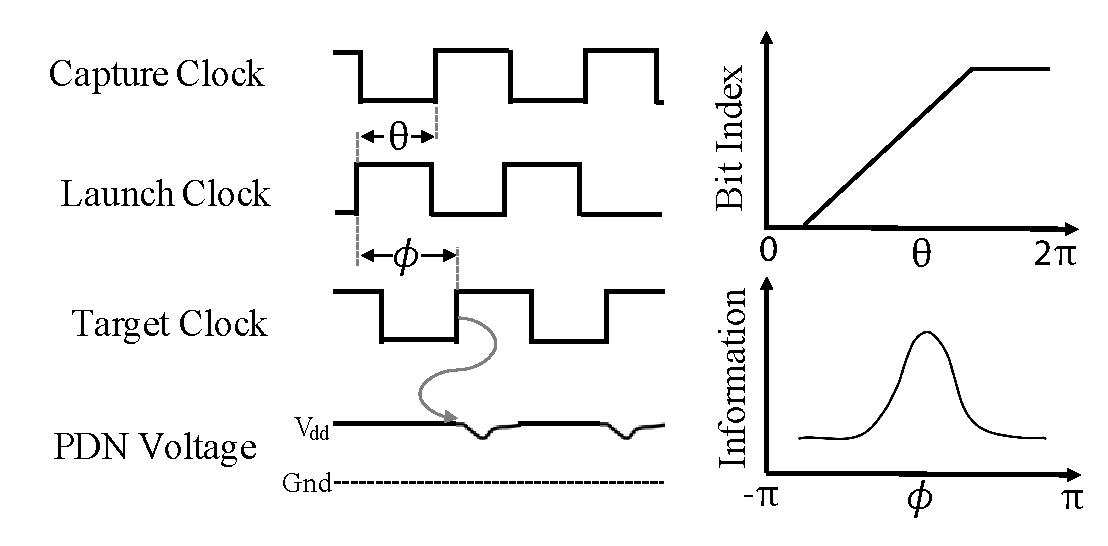
\includegraphics[scale=.55]{img/phi-theta.pdf}
\vspace{-10px}
\caption{Tuning Parameters for our Tunable TDC Sensor. $\phi$ and $\theta$ define the relationship between the launch, capture and target clocks in our \name TDC. $\theta$ is the known phase relationship between the launch and capture clocks and affects the location of the transition bit index. $\phi$ is the unknown phase relationship between the launch and target clock. Variations in PDN voltage are caused by power consumption around the positive edge of the target clock. 
\textit{Tuning} is the process of searching for $\phi \to 0$ such that power variations maximize the extracted information.
}
\label{fig:phi-theta}
\vspace{-10px}
\end{figure}